%! Author = melek
%! Date = 22.01.2023

% Preamble
\documentclass[11pt]{article}

% Packages
\usepackage{amsmath}
\usepackage{graphicx}
\graphicspath{ {../images/} }

\title{Assignment 4: Model Based RL}
\author{huseyinabanox@gmail.com}
\date{January 2023}

% Document
\begin{document}

    \maketitle

    \section*{Problem 1}

    \subsection*{First Run}

    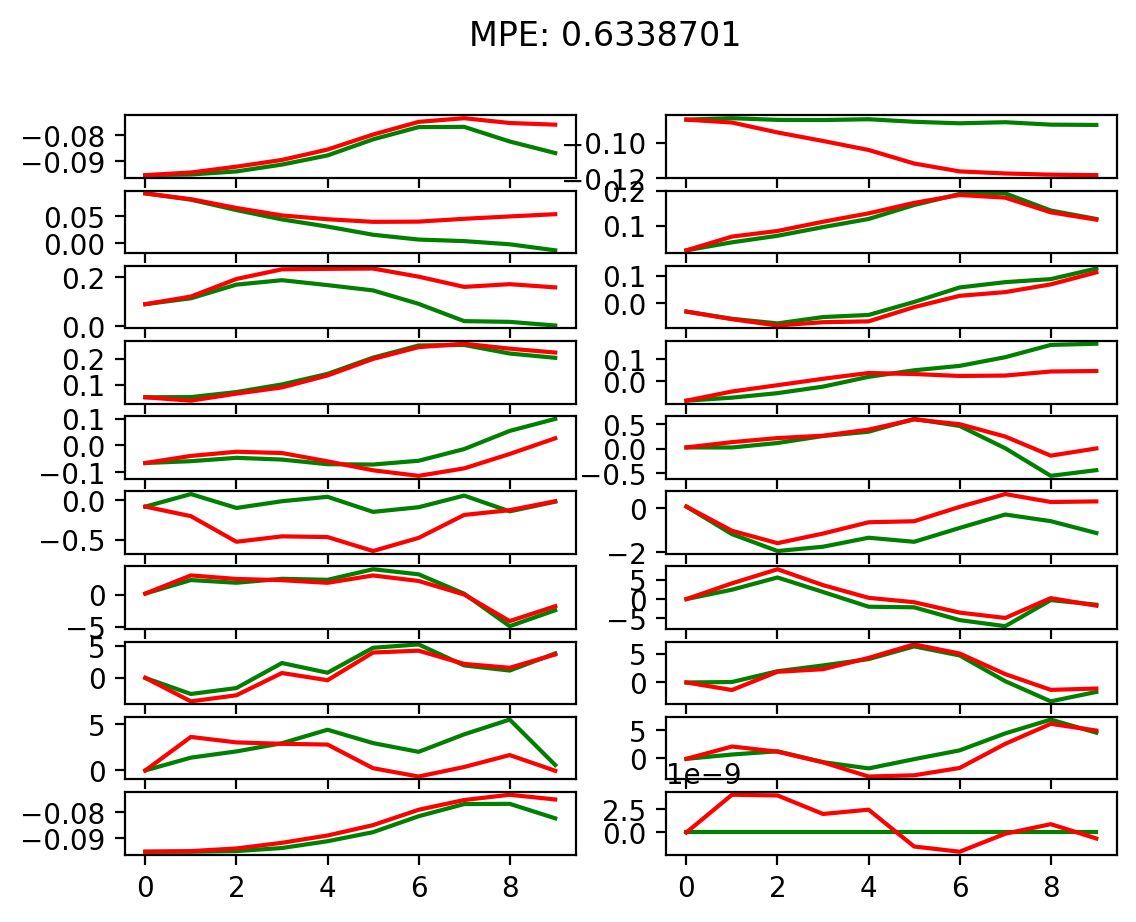
\includegraphics[scale=0.9]{q1/itr_0_predictions_run0}

    A small network is used.
    Results can be improved using a larger network.

    \subsection*{Second Run}

    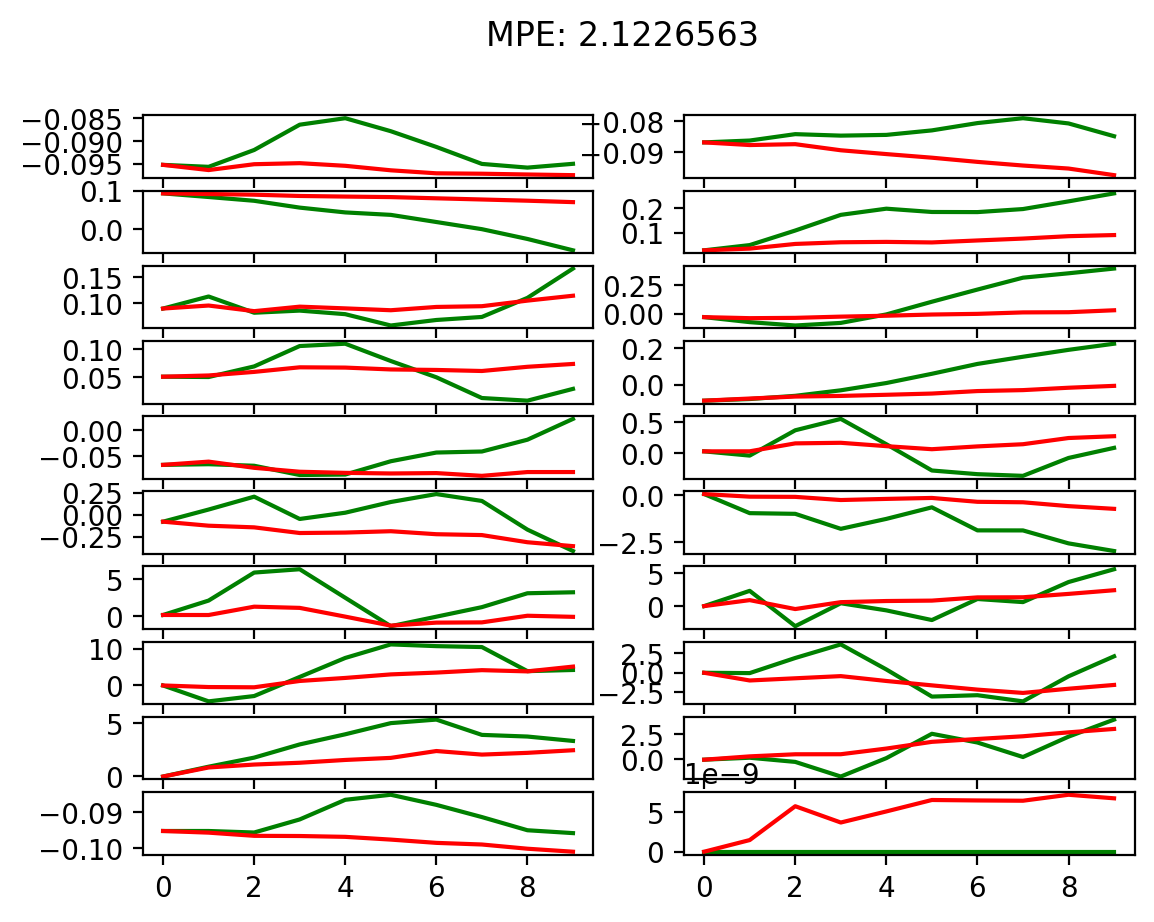
\includegraphics[scale=0.9]{q1/itr_0_predictions_run1}

    Small number of iterations are used.
    Results can be improved by increasing iteration count.
    MPE is the worst.

    \subsection*{Third Run}

    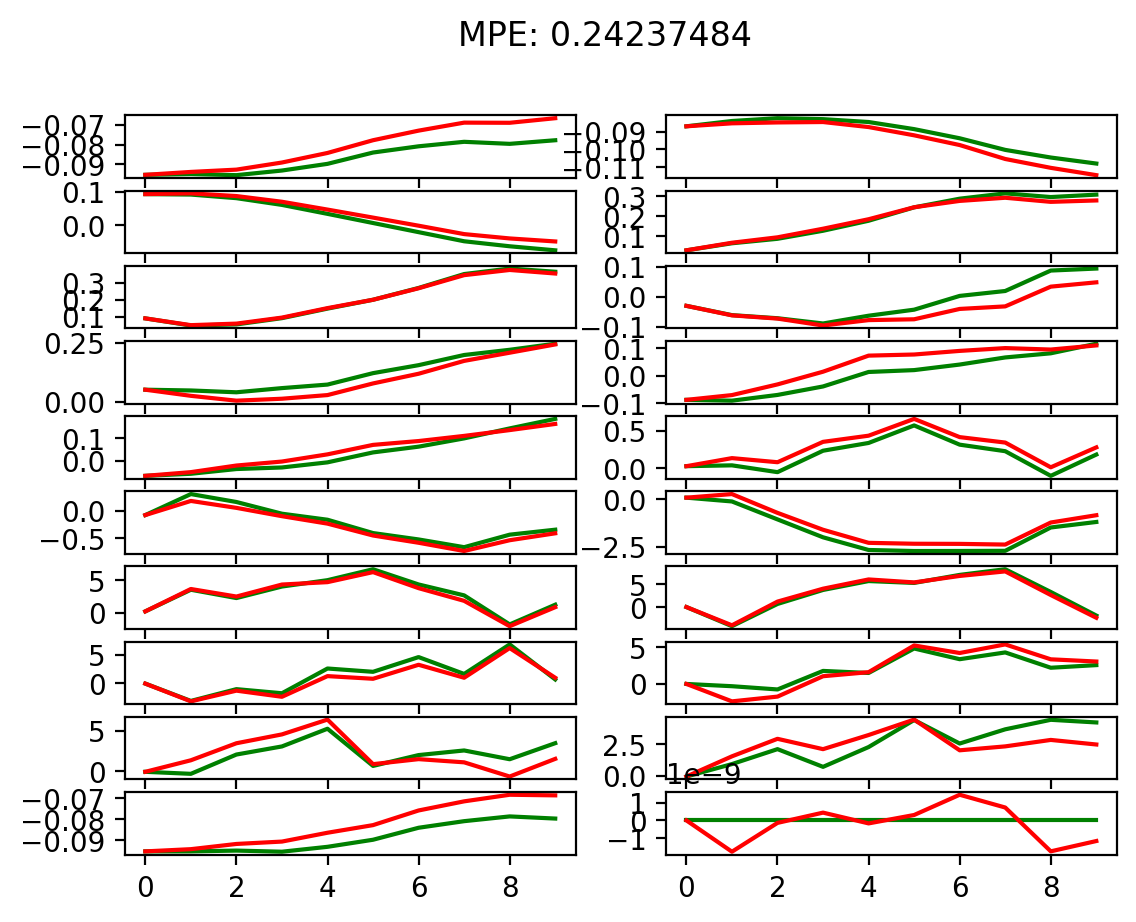
\includegraphics[scale=0.9]{q1/itr_0_predictions_run2}

    Best results are obtained using a larger network and more iterations.
    MPE is the best.

    \section*{Problem 2}

\end{document}